\documentclass[letterpaper]{article}

\usepackage{graphicx}
\usepackage{url}
\usepackage{float}

\title{Does the Version Control System affect commit understandability?}
\author{Mihai Codoban \and Caius Brindescu}
\date{}

\begin{document}

\maketitle

\section{Research questions}

\begin{enumerate}
	\item Do SVN commits take more time to understand than Git commits?
	\item Does user background (programming experience, industry experience etc) influence the time it takes to understand a commit?
	\item Does user background influence the quality and depth of the understanding of a commit or change description?
	\item Is there a common leave of change description between people?
\end{enumerate}

\section{Method}

\subsection{Participants}

Our participants are Java developers with Version Control Systems (VCS) experience. 
This includes:
\begin{itemize}
	\item at least 5 years of programming experience
	\item at least 1 year of experience using Java
	\item at least 1 year of experience using a VCS
\end{itemize}

Participants are recruited via email lists, university announcements (electronic and billboards), and local software companies targeting.

The study involved 30 participants (5 people x 6 sessions). 
We recruited 47 people (30 participants, 2 no-shows per session and 5 pilots).

\subsection{Apparatus or Materials}
\label{apparatus}

Participants will be viewing commits in a custom made software that for each commit shows the commit message, the diff (using the Eclipse Comparator Editor) and a text box where the commit description would be written.
They will have the following materials:
\begin{itemize}
	\item checklist of items to look for when understanding commits (embedded in commit window)
	\item commit information (commit message and commit diffs)
	\item questionnaire
\end {itemize}

Each participant described 3 SVN commits and 3 Git commits.
Each commit is chosen from a different repository.
Repositories are chosen from the top 6 Java repositories.
We selected 3 repositories using Git from GitHub and 3 repositories using SVN from SourceForge.
A commit is randomly chosen from the last commits in a project.
We believe this the last commits are representative of the change done in the later stages of the development.
To ensure the integrity of the commits we ignore commits that 
\begin{itemize}
	\item Contain changes to non-Java source files (build scripts, configuration files, etc);
	\item Are merge commits (this applies for Git only);
	\item Only change the formatting or comments.
\end{itemize}

The post study questionnaire included the following questions: 
\begin{itemize}
	\item{Programming experience}
	\item{Java Experience}
	\item{Type of projects they work on}
	\item{VCS paradigm preference}
	\item{VCS use}
	\item{VCS experience}
	\item{Commit frequency}
	\item{Commit composition strategy}
\end{itemize}

\subsection{Procedure}

This will be a within subjects study. 
Each participant has to understand and describe 3 SVN commits and 3 Git commits. 
The order in which we apply the treatments is random for each participant. 
This is done to eliminate the learning effect. 

The following script will be followed for each session:
\begin{enumerate}
	\item Informed Consent
	\item Administer tutorial
	\begin{enumerate}
		\item Explain the UI
		\item Explain the tasks to the participants
		\item Do a demo task
	\end{enumerate}
	\item Practice Task
	\item Study Tasks
	\begin{enumerate}
		\item Each task contains the commit message and the commit changes.
		\item The participant has to understand the commit. We provide a checklist of items to check
		\item The participants are instructed to maximize detail
	\end{enumerate}
	\item Administer post session questionnaire
	\item Pay participants and receive receipts 
\end{enumerate}

\section{Data}

For each participant, we will collect the following:
\begin{enumerate}
	\item Time when they start a task
	\item Time when they complete a task
	\item The description of the commit
	\item Timestamp of all the key presses.
	\item Post-session questionnaire
\end{enumerate}

The time needed to understand a commit is determined by subtracting from the time it took to complete a task, the time it took the participants to type in their answer.
This will eliminate any variation due to varying typing speeds.
This variation can be seen in figure \ref{fig:typingTimes}.

In order to subtract the typing time a threshold needs to be set up to differentiate between real typing and thinking pauses.
For the threshold we used the mental preparation constant (1.2 seconds) from the KLM model \cite{klm}.

\begin{figure}[H]
    \centering
    \includegraphics[width=0.7\textwidth]{../data/analysis/typingTime.pdf}
    \caption{Variation between participant typing times. The time for each participant is computed by averaging all the participant's task times.}
    \label{fig:typingTimes}
\end{figure}

\section{Results}

\subsection{RQ1: Is the commit understanding time influenced by the VCS?}

%how data looks
To answer this research question we looked at how long it took participants to understand commits.
Each participant produced 6 understand times, 3 for SVN and 3 for Git.
For each participant we averaged the SVN times and Git times thus obtaining two times for the two VCS tools.
We then separated these times in two bins: one bin of SVN times and one bin of Git times. 
The averaging of times per participant was done so as not to have related data (more times from the same participant) in the same bin.
Figure \ref{fig:rq1-data} shows how we arranged the data.

\begin{figure}[H]
    \centering
    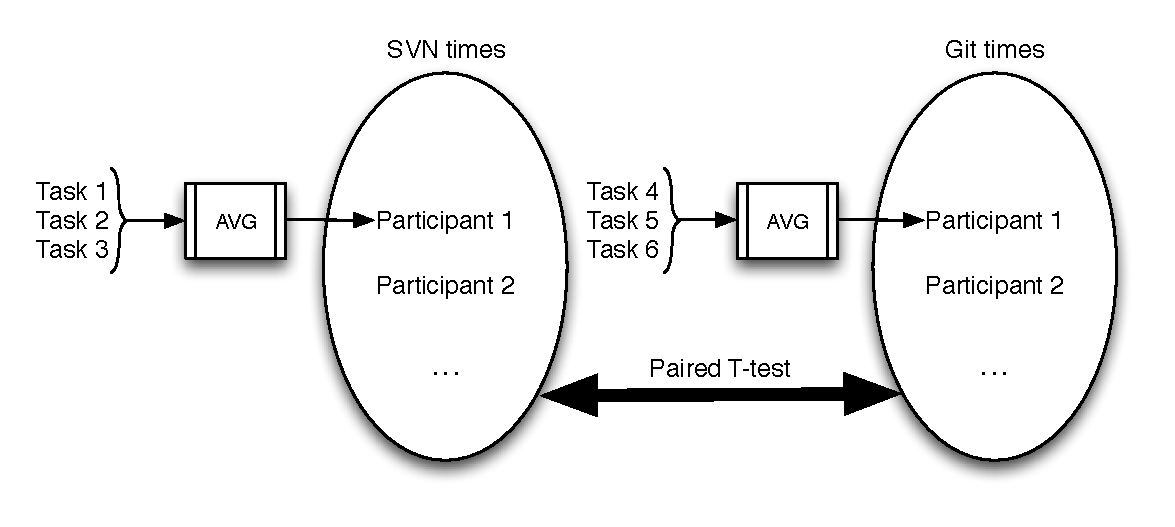
\includegraphics[width=0.9\textwidth]{fig/RQ1-data}
    \caption{RQ1 data aggregation. Tasks 1, 2 and 3 represent the SVN tasks whereas tasks 4, 5 and 6 represent the Git tasks.}
    \label{fig:rq1-data}
\end{figure}

%what test we used on this data=
To test whether the SVN times are different from Git times we performed a paired T-test.
The test is paired because one SVN data point is connected to one Git data point by the fact that they come from the same participant.
We thus tested whether participants require different times to understand commits under different VCS tools.

%results of test
The test returned a significant result (t = 11.535, df = 29, p-value = 2.352e-12). 
We can thus reject the null hypothesis that there is no difference between participants' understand time of SVN and Git commits.
The participants took a longer time to understand SVN commits by an average of 2.23 minutes.

%show plots and describe data 
Figure \ref{fig:rq1-participantTimes} shows the understand times for each participant, grouped by SVN and Git.
It is visible that all participants tended to understand Git commits in less time than SVN commits.

Participant P1 has lower understand times than the rest.
This is due to the fact that P1 was exposed to a tutorial that did not clearly state that depth of understanding is required.
We therefore changed the tutorial for the rest of the participants.
This change produced consistent times for participants P2, P3, P4 and P5.
However, even P1 showed a difference in the understand times between the two VCS tools.

\begin{figure}[H]
    \centering
    \includegraphics[width=0.6\textwidth]{../data/analysis/RQ1_ParticipantTimes}
    \caption{Participant understand times for SVN and Git. Red represents SVN tasks and green Git tasks.}
    \label{fig:rq1-participantTimes}
\end{figure}

Figure \ref{fig:rq1-taskTimes} shows the understand times grouped by tasks.
It can be seen that, overall, SVN tasks took a longer time to understand than Git tasks.

\begin{figure}[H]
    \centering
    \includegraphics[width=0.6\textwidth]{../data/analysis/RQ1_TaskTimes}
    \caption{Task understand times. Red represents SVN tasks and green Git tasks.}
    \label{fig:rq1-taskTimes}
\end{figure}

%interpretation

\textbf{Interpretation}

The difference in times can be accounted for by the differences between Git and SVN. 
Prior research \cite{brindescu2014centralized} on the differences between Distributed and Centralized Version Control paradigms found that DVCS users can perform smaller commits that contain one cohesive intent of change rather than a code dump.

This is due to the fact that DVCS users (i) can work in isolation on local copies of the repositories enabling them to work offline while still retaining full project history, (ii) they can cheaply create and merge branches, and (iii) they can commit individual changed lines in a file, as opposed to being forced to commit a whole file like in CVCS.

These differences lead to commits that may be easier to understand and reason about.
The results from RQ1 support this hypothesis.
Instead of the repository being a series of code dumps, Git repositories are more similar to a series of commits that each tell a cohesive story on how the software evolved.

\subsection{RQ2: Does the user background (programming experience, etc) influence the time it takes to understand a commit?}

In order to gather participant background we used a post study questionnaire (more details in section~\ref{apparatus}).

We answer RQ2 by searching whether there is any questionnaire item that influences participants' commit understand time.

For each participant, we averaged all the understand times, indifferent of the VCS tool.
Thus we obtained a global understand time for each participant.
In this research question we ignored the data from participant P1 since he was an outlier, as figures~\ref{fig:rq1-participantTimes}~and~\ref{fig:rq2-understandTimes} show.

We ran ANOVAs that considered the questionnaire questions as being the independent variables (the treatment) and the participant understand times (1 for each participant) the dependent variable.
Although all questions were found to have a significant influence (P \textless{} 0.05) on the understand time, the mean differences were about 30 seconds.

This difference is meaningless.
We measured the understand time by subtracting the typing time from the total time of the task.
Since this is a coarse grained measurement, small time intervals are meaningless because participants may loose focus at random places in time.
Moreover, the understand times of participants P2, P3, P4 and P5 are very consistent, as figure~\ref{fig:rq2-understandTimes} shows. 
This again renders any small differences meaningless.

\textbf{Interpretation}

%commit understanding is similar to reading, therefore we hypothesized that they would be influences only by experience
We assume that commit understanding is similar to program comprehensions, since both require reading and making meaning of code.
We also assume that programming and language experience would influence program comprehension speed and thus commit understanding.
Therefore we hypothesized that only these two experiences would influence the understand time of the participants in our study.

%but we found out that there are meaningless differences due to the fact everybody is the same
However, we found out that all questionnaire questions cause significant but meaningless differences.
This could be due to the fact that our participants were very similar to each  other both in terms of background and in terms of understand time.
Thus any difference, however meaningless, would appear significant.

%to properly answer this questions we would have to obtain a more representative sample that covers all dev categories
The participants were almost homogeneous in terms of programming and Java experience.
To answer this research question in a valid way we would need to perform a different study in which we actively sample the population in such a way that we obtain participants from all categories (experienced, inexperienced, java developers, non java developers, etc)

\begin{figure}[H]
    \centering
    \includegraphics[width=0.6\textwidth]{../data/analysis/RQ2_AllUnderstandTime}
    \caption{Average understand times for each participant. The bottom outlier is participant P1.}
    \label{fig:rq2-understandTimes}
\end{figure}


\subsection{RQ3: Does the user background influence the quality and the depth of understanding a commit or a change description?}
\label{sec:RQ3}

%how data looks
For this and the next research question we graded the commit description.
We used a grading rubric that noted how many changes participants found in a commit and how deep they detailed them.
For each task we normalized that task's grades in the following manner: $ [0, MaxTaskGrade] \mapsto [0, 10]  $.
Normalization allows to compare grades between tasks.

For RQ3 we used the same data structuring as in RQ2.
The only difference is that we swapped the understand time with the commit description grade.
Thus for each participant we computed an average grade and explored whether any questionnaire items affect participants' grades.

%what test we used on this data
%results of test

Similar to RQ2, we ran ANOVAs with the questionnaire items as independent variables and the grade as the dependent variable. 
We discovered that participants' answers to the VCS usage and the VCS paradigm preference questions (see section \ref{apparatus} for questionnaire details) cause a significant difference in the participant grade (P \textless{} 0.05).

We then performed two T-tests with the VCS usage and VCS paradigm preference as independent variables and the participant grade as the dependent variable.
Both tests showed a significant difference with (p = 1.99e-12, t = -14.78, df = 26.89) for VCS usage and (p = 1.01e-12, t = -11.50, df = 18) for VCS preference.

Tables~\ref{tab:rq3_vcsUsage}~and~\ref{tab:rq3_vcsPreference} show the grade difference between the two question groups.
Participants who answered with Git for the VCS usage question and with Distributed for VCS paradigm preference got lower grades than participants who answered with SVN and No Preference respectively.

\begin{table}[H]
	\centering
	\begin{tabular}{c | c c c c}
										& Git  & SVN \\ \hline
	Average grade & 3.63 & 7.71
	\end{tabular}
	\caption{Average grades for participants who responded with Git and SVN for the question referring to VCS usage.}
	\label{tab:rq3_vcsUsage}
\end{table}

\begin{table}[H]
	\centering
	\begin{tabular}{c | c c c c}
							& Distributed Paradigm  & No Preference \\ \hline
	Average grade & 2.97 & 6.8 
	\end{tabular}
	\caption{Average grades for participants who responded with Distributed and No Preference for the question referring to VCS paradigm prefence. There were no responses for the Centralized paradigm.}
	\label{tab:rq3_vcsPreference}
\end{table}


%show plots and describe data 

%interpretation

\textbf{Interpretation}

%could be experience ... but all of them are the same
As with RQ2 and for the same reasons, we hypothesized that the only background attributes that would influence the grade are programming and Java experience.
Instead, it appears that the participants' declared choice of VCS tool and paradigm influenced the grade and not their experience.

One explanation would be that VCS tool and paradigm preference may be confounded with experience.
But our participants are almost homogeneous in terms of experience, so experience is not a confounding factor.

%could be the threat
Several participants raised the issue that the VCS tool and paradigm preference questions were ambiguous.
They claimed that it was not clear whether the questions' scope included their whole lifetime or only their latest experiences.
Therefore the results for this research question may not be valid.

%open question; more research needed
To answer this question another study is needed in which the focus is on the survey and population sampling.
The sampling would need to capture participants of all experiences and VCS preferences in order for this question to be answered in a reliable and valid manner.

\subsection{RQ4: Is there a common level of change description between people?}
\label{seq:rq4}

%how data looks
For this research question we structured the data in the same manner like RQ1 (figure~\ref{fig:rq1-data}).
The difference is that instead of using the understand time as the dependent variable, we used the normalized grades (see section \ref{sec:RQ3} for grading details).

%what test we used on this data
To answer this research question we look at the grade distribution in order to see how the common grades look like (and thus, the common level of description).
We then further explore the question by looking into the difference between SVN task grades and Git task grades by means of a T-test.

%results of test
%show plots and describe data 
Figures~\ref{fig:rq4-allParticipantsBox}~and~\ref{fig:rq4-allParticipantsHist} show that the grade distribution is marginally normal.
More data points are needed though for a reliable answer.
The boxplot shows that on average participants caught half of the commit details.

\begin{figure}[H]
    \centering
    \includegraphics[width=0.6\textwidth]{../data/analysis/RQ4_AllGradesBoxPlot}
    \caption{Participant grades boxplot.}
    \label{fig:rq4-allParticipantsBox}
\end{figure}

\begin{figure}[H]
    \centering
    \includegraphics[width=0.6\textwidth]{../data/analysis/RQ4_AllGradesHistogram}
    \caption{Participant grades histogram.}
    \label{fig:rq4-allParticipantsHist}
\end{figure}

The T-test between participants' SVN and Git grades did not return a significant result (p=0.09; t=1.76; df=24). 
For a confidence level of 0.95 we cannot reject the null hypothesis that there is no difference between participants' grades for SVN and Git commits.
However, there is a marginal difference between the two groups with SVN grades being 0.28 higher on average.
We do not consider this difference meaningful.
Figures~\ref{fig:rq4-participantGrades}~and~\ref{fig:rq4-taskGrades} show the marginal tendency of higher SVN grades.

\begin{figure}[H]
    \centering
    \includegraphics[width=0.6\textwidth]{../data/analysis/RQ4_ParticipantGrades}
    \caption{Individual participant grades, grouped by SVN (red) and Git (green) tasks.}
    \label{fig:rq4-participantGrades}
\end{figure}

\begin{figure}[H]
    \centering
    \includegraphics[width=0.7\textwidth]{../data/analysis/RQ4_AllGrades}
    \caption{Average task grades. SVN tasks are marked with red and Git tasks are marked with green.}
    \label{fig:rq4-taskGrades}
\end{figure}

\textbf{Interpretation}

RQ3 and RQ4 show a marginal tendency of SVN grades to be higher than Git grades.

%why are git grades lower 
We have two hypotheses why this would be so:
\begin{enumerate}
		\item{Biased grading rubric.}
			Our grading rubric awarded points both for mentioning changes and for detailing the changes as well.
			It may be that since Git commits tend to be shorter, simpler and more cohesive the participants felt no incentive to detail an already easy and small change.
			On the other hand, since SVN commits are large, complex and unrelated it may be that participants felt the need to detail them more thoroughly.
			This would inherently lead to higher SVN grades with our grading rubric.
	\item{Exaggerated Cost / Benefit Analysis.}
			When participants see a big commit, they might prepare themselves mentally for a huge workload, therefore they catch more commit changes and thus a higher grade. 
			On the other hand, when participants see a small commit, they adopt a low mental preparation therefore they catch less commit changes and thus a lower grade.
\end{enumerate}

%how this could affect RQ1
The results of RQ4 and RQ3 made us revisit RQ1 and take into consideration the grade as a confounding variable.
If participants get lower grades for Git commits, then this may lead to smaller understand times for Git commits.
We ran an ANOVA with intercepts in which we considered the understand time as a dependent variable and the commit origin and the commit grade as the independent variables.
Table~\ref{tab:rq4_anovas} shows that both independent variables influence the understand time.
The interaction between commit origin and commit grade on the other hand does not influence the understand time.
On the other hand this model explains only 40\% (R squared) of the variation in understand time.

\begin{table}[H]
	\centering
	\begin{tabular}{c | c c c c}
													& DF	&	Mean sq	&	F value	&	Pr(\textgreater F)	\\ \hline
	Commit Origin							& 1	&	74.51		&	22.77	&	1.35e-5					\\ 
	Commit grade							& 1	&	65			&	19.87	&	1.03e-5					\\
	Commit Origin : Commit grade	& 1	&	2.2			&	0.63	&	0.41						\\
	\end{tabular}
	\caption{Influence of the VCS tool and the commit grade on the understand time.}
	\label{tab:rq4_anovas}
\end{table}

\section{Discussion}

Our lab study shows that commits originating in Git take less time to understand than commits originating in SVN and that the understand time does not depend on participant background.

Participants tend to capture about half of commit details on average with our data hinting that the grade distribution may be normal (although a larger sample size would provide a definite answer).

Most surprisingly, commit grades marginally tend to be higher for SVN commits.
This finding is supported by two sources: the actual SVN and Git grades from the lab study and the correlation between participant background and commit grades.
On the other hand, for the lab measurements we do not consider the grade difference as being meaningful (as section \ref{seq:rq4} shows).

%difference in repository structure and behaviour. further research to build a concrete theory of VCS impact on repo structure and dev behaviour
These results support the theory that developers' change management behaviour varies with the VCS tool.
We think the results represent yet more evidence that warrants deeper research into how VCS tools impact repository structure and developer behaviour.

%interesting ideas about change understanding
The difference  between SVN and Git grades remains an open question.
Our best assumption is that the cause lies within the field of developer cognitive models in the task of program (and program change) comprehension.

\subsection{Threats to validity}

\subsubsection{Internal Threats}

\paragraph{Maturation.}
The participants had to describe a total of 6 commits.
Some participants complained that this activity was hard and boring.
Therefore there is the risk that participants' effort of understanding decreased with time.
We mitigate this risk by randomizing the order in which each participant received the tasks.

\subsubsection{External Threats}

\paragraph{Commit Selection.}
While the commits were selected randomly, there is a possibility that they are not representative for the general practice.
Projects have thousands of commits and we randomly chose one from each project.
We tried to pick typical code change commits by choosing from the last commit in a project and filtering noisy commits.

\paragraph{Tool.}
For this study we build a special tool. 
This might be different than the tools used in the wild.
However, for representing the commits we chose the standard Eclipse commit viewer.
This is a well known graphical model of viewing commits.

\paragraph{Selection.}
In terms of the population, our results are representative of experienced programmers an experiences VCS users.
We do not know how the lack of experience might impact commit u

\subsubsection{Construct Threats}

\paragraph{Personal bias of understanding.}
The participants had to self-assess when they understood all the changes. 
This varies from person to person. 
Offering a checklist and grading the responses tried to mitigate this risk as much as possible.

\paragraph{Measuring understanding.}
We measured the understanding time by subtracting the typing time from the total task time.
This subtraction is due to different typing times for different people.
However, except the typing time, participants may not have been mentally engaged in the task at all times.

\paragraph{Biased Grading Rubric.}
Our grading rubric takes into account both the quantity of mentioned changes and their depth of detail as well.
Since Git commits may be smaller, simpler and more cohesive in contrast to SVN commits, participants may be inclined to only mention Git changes and not detail them.
This would inherently lead to larger grades for SVN commits.

\paragraph{Ambiguous survey question.}
The survey question involving VCS use and preference was reported as being ambiguous.
Participants were not sure whether to respond with their latest preferences or with their overall experience.

\subsubsection{Reliability Threats}

The details described in this paper are sufficient to recreate the experiment.
Moreover the source code of the tool, collected data, analysis scripts and the survey are publicly available\footnote{\url{github.com/cdmihai/CS589}} \footnote{goo.gl/uZM5vL}.

% Bibliography
\bibliographystyle{abbrv}
\bibliography{report} 

\end{document}